\def\GelfandBasisLabel{баз... [?]}
\begin{center}
\begin{minipage}[t]{.46\linewidth}\vspace{0pt}\centering
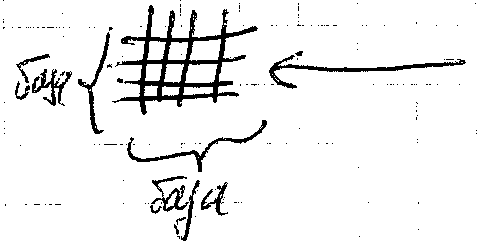
\includegraphics[width=\linewidth]{figures/gelfand-0153-p001412-basis-grid-original.png}\par\smallskip
{\footnotesize Оригинал рукописного рисунка: \texttt{GELFAND-P001412}}
\end{minipage}\hfill
\begin{minipage}[t]{.50\linewidth}\vspace{0pt}\centering
{\footnotesize Частичное воссоздание видимых штрихов}\par\smallskip
\resizebox{\linewidth}{!}{\begin{tikzpicture}[x=.75cm,y=.75cm]
\foreach \x in {0,.28,.56,.98}{\draw (\x,-.1)--(\x+.09,1.1);}
\foreach \y in {0,.15,.38,.67}{\draw (-.16,\y)--(1.26,\y+.06);}
\draw (-.3,1.05) .. controls (-.35,.8) and (-.42,.59) .. (-.56,.54)
 .. controls (-.36,.5) and (-.52,-.1) .. (-.35,-.15);
\draw (-.12,-.3) .. controls (-.31,-.71) and (.45,-.31) .. (.52,-.6)
 .. controls (.57,-.31) and (1.19,-.55) .. (1.35,-.18);
\node[left] at (-.58,.5) {\GelfandBasisLabel};
\node[below] at (.6,-.68) {\GelfandBasisLabel};
\draw[->] (2.97,.45)--(1.43,.43);
\end{tikzpicture}
}
\end{minipage}
\end{center}
\noindent{\small\textit{В обеих подписях скобок сохранено лишь начало «баз...»; окончания не установлены после просмотра при 3×, 5× и 10×. Термины базисов строк и столбцов не определяют начертание.}}
